\subsection{Recording}
Recording is the process of collecting and storing physiological signals from sensors over an extended period. To enable a recording, we need to establish a connection with the available sensors and store the samples retrieved by the sensors on the device. We will use the Data Stream Dispatching Module (hereafter: DSDM) which manages sensor discovery and sensor establishment to supported sensor sources. DSDM facilitates an interface for data acquistion, and the communication between the DSDM and Nidra occurs over IPC. Moreover, we will implement functionality to check for connectivity during record, to ensure the sensors are collecting data to at appropriate rate. At the end of recording, we will store metadata related to the recording session and finialize the recording process. 


The functionality of recording can be divided into three actions: (A) start a recording; (B) stop a recording; and (C) display recording analytics. In the following Subsection for recording, we will review the steps to enable these actions. 

\subsubsection{Action A: Start a Recording}
\begin{figure}
    \centering
    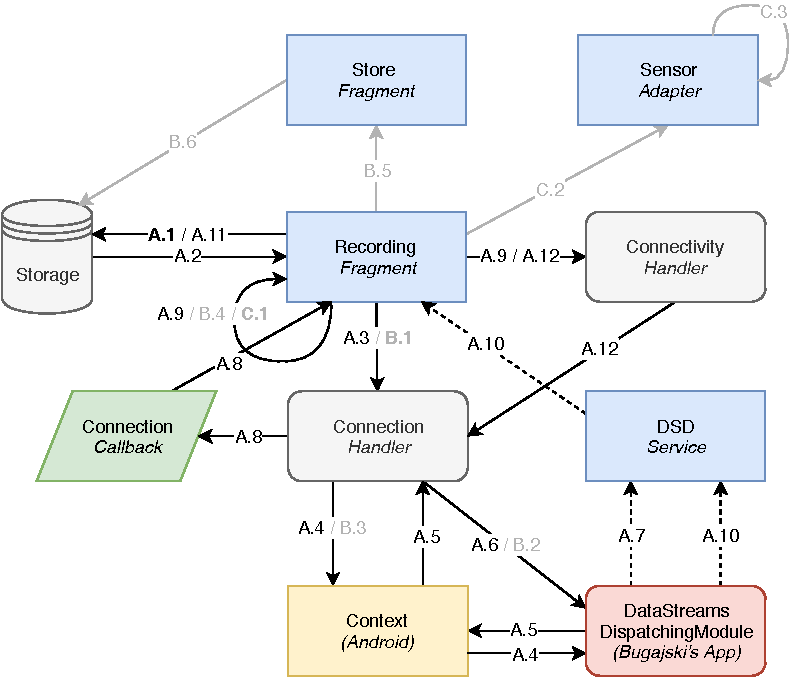
\includegraphics[scale=0.7]{images/Recording_ImpA.pdf}
    \caption{Implementation of recording functionality: (A) Start a Recording}
    \label{fig:impl_recordingA}
\end{figure}

In Figure \ref{fig:impl_recordingA}, an illustration of the component interactions are shown. Action A is to start a recording by connecting and starting data aqusition with the use of DSDM, and to ensure persistent connectivity with the sensor sources. The steps and interactions for this action are: 

\begin{itemize}
    \item[A.1] Commence the recording by creating a record entity and inserting it into the database. An empty record has to be inserted into the database in order to associate new samples to the recording. 
    \item[A.2] Once the record is inserted into the storage, unique identification is returned. 
    \item[A.3] \verb|ConnectionHandler| manages the establishment, connection, and disconnection of the IPC between Nidra and DSDM. It starts by establishing a connection to the DSDM:
\begin{lstlisting}[language=json, caption={My Caption}, captionpos=b]
    Intent intent = new Intent(MainServiceConnection.class.getName());
    intent.setAction("com.sensordroid.ADD_DRIVER");
    intent.setPackage("com.sensordroid");
    context.bindService(intent, serviceCon, Service.BIND_AUTO_CREATE);
\end{lstlisting}
    \verb|MainServiceConnection| is the AIDL file (discussed in IPC).
    \item[A.4] We bind to service by using the \verb|BindService|. If the service is offline, the flag \verb|Service.BIND_AUTO_CREATE| will ensure the service is started. \verb|BindService| allows components to send requests, receive responses, and perform inter-process communication (IPC) [CITE]. 
    \item[A.5] Once the service has bound, we can proceed to communicate with the DSDM. 
   	\item[A.6] The \verb|ConnectionHandler| proceeds to initialize the connection with the sensor through the DSDM.  A request to the DSDM for available publishers with \verb|getPublishers()| is made, to retrieve all available sensor publishers connected to the DSDM. Occasionally, the DSDM uses extended time to discover all of the active sensors connected to the device; therefore, we have an interval that checks whether DSDM has any available sensors connected.
	\item[A.7] Moving on,  a request to the DSDM to \verb|Subscribe| to a sensor is made.  In the \verb|Subscribe| function, a reference to the package name and a service object (\verb|DSDService|) from Nidra is sent. The service object is where all of the parcels of data from the DSDM is received.   
	\item[A.8] A callback to \verb|RecordingFragment|  with the available sensor publishers is made. 
	\item[A.9] The recording has now started, and a timer to measure the time spent on the record is started. 
	\item[A.10] The \verb|ConnectivityHandler| is the component we discussed in Section ... , which checks for sample arrival and activity to reconnect with the sensor. The \verb|ConnectivityHandler| is implemented with a \verb|Handler| with a \verb|PostDelay|. If the event for the \verb|PostDelay| is triggered, it is equivalent for a sample not being acquired from the sensor. 
	\item[A.11] Periodically, the DSDM receives samples from the subscribed sensor. DSDM forwards the sample from the sensor to the service object (\verb|DSDService) on the \verb|putJson| function. The DSDService uses a \verb|LocalBroadcastManger| to send bundles of data across components in the application. The \verb|RecordingFragment| is listening for the event, and receives all of the data. 
	\item[A.12] The data received from the sensor (through the DSDM, to DSDService, and LocalBroadcast), is stored as a new sample entry with the current recording identification associated with it. 
\end{itemize}

\subsubsection{Action B: Stop a Recording}
\begin{figure}
    \centering
    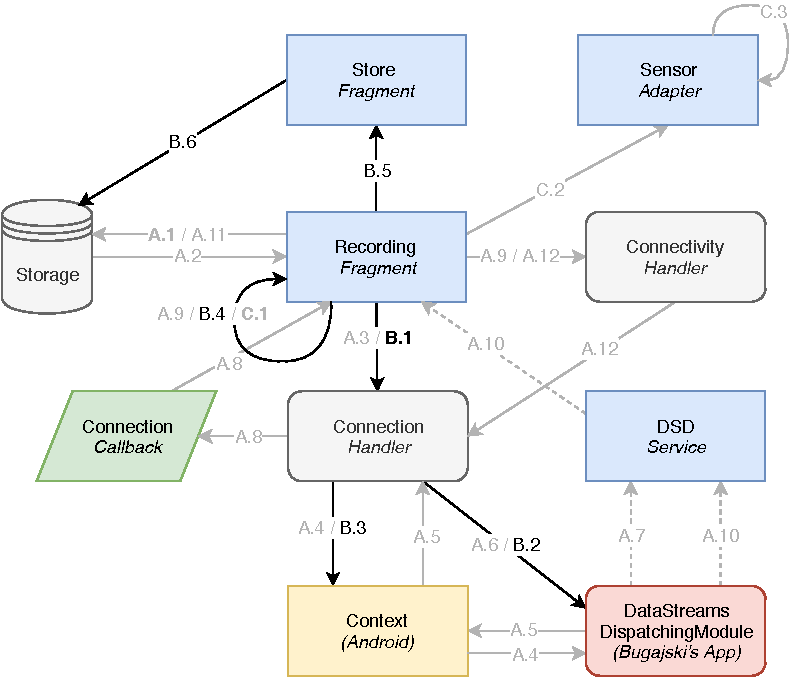
\includegraphics[scale=0.7]{images/Recording_ImpB.pdf}
    \caption{Implementation of recording functionality: (B) Stop a Recording}
    \label{fig:impl_recordingB}
\end{figure}

In Figure \ref{fig:impl_recordingB}, an illustration of the components to stop a recording is shown. The action is based on the user input to stop the recording session. For the user, the recording has terminated and the user is presented with a screen to provide information regarding the recording (e.g., title, description and rating). For the application, has to notify and unsubscribe to the connected sensors through DSDM, as well as disconnect from the DSDM service. In addition, manage the metadata the user provides at the end of the recording session, and storing recording metadata on the device. The steps and interaction for this action are:

\begin{itemize}
	\item[B.1] The user of application decides when to stop a recording with a press of a button. The event to stop recording is sent to the \verb|ConnectionHandler|.
	\item[B.2] A call to the \verb|Unsubscribe| function on the subscribed subscribe with the service object is sent to the DataStreamsDispatchingModule (hereafter: DSDM). The DSDM has to ensure to unsubscribe unpublish the sensor in order to signal the sensor to stop sampling. 
	\item[B.3] The IPC connection between Nidra and DSDM is discontinued by unbinding the service. 
	\item[B.4] The estimated time of recording is calculated, and a transition from \verb|RecordingFragment| to \verb|StoreFragment| is made to finalize the recording with extra information (e.g., title, description, and rating). 
	\item[B.5] The \verb|StoreFragment| uses the record identification retrieved on recording (A.1) in order to enrich the record with statistics and user-defined metadata. The statistics are the monitoring time, number of samples during recording, and retrieving the current state user biometrical data and storing it in the record. The user-defined metadata are the title of the recording, a description enabling the user to add a note to the recording, and a rating between 1--5 (to give a rating on how the recording felt). 
	\item[B.6] The modified record is updated in the database, and the user is transitioned to the \verb|FeedFragment|.
\end{itemize}


\subsubsection{Action C: Display Recording Analytics}
During a recording, the user can view the analytics for the recording. More spesifically, the user can see the available connected sensors, and a graph of respiration (based on the samples acquesitions from the sensor) in real-time. In Figure \ref{fig:impl_recordingC}, an illustration of the components display recording analytics is shown, and the steps and interaction for this action are: 

\begin{figure}
    \centering
    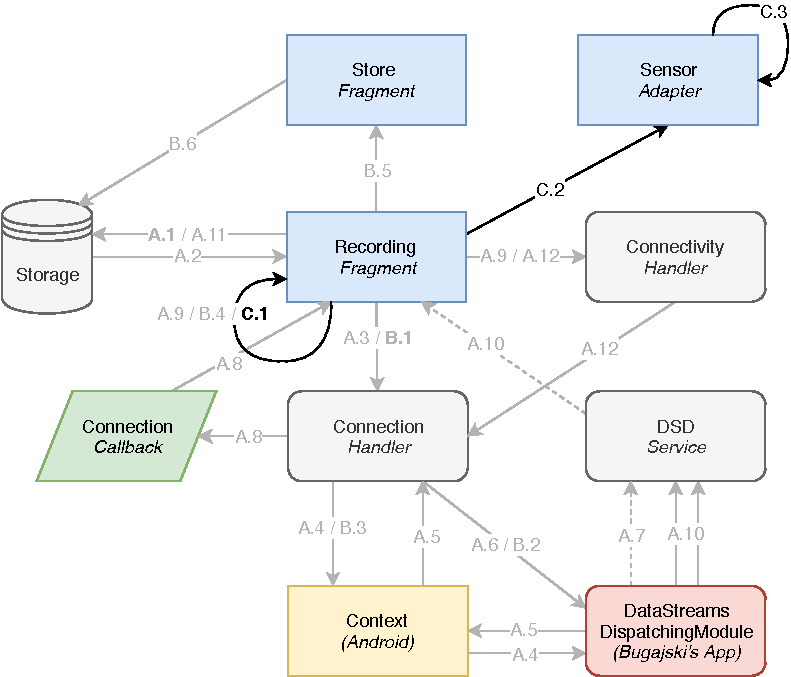
\includegraphics[scale=0.7]{images/Recording_ImpC.pdf}
    \caption{Implementation of recording functionality (C)}
    \label{fig:impl_recordingC}
\end{figure}

\begin{itemize}
    \item[C.1] The data is graphically represented as an intractable time-series graph. By using the Graph library, we can in similarities to the implementation of the analytics concern (see Subsection), implement a graph to illustrate the respiration data to the user.
    \item[C.2] In addition to the time-series graph, we have a list of sensors that are sampling in the recording. 
    \item[C.3] The \verb|Sensor Adapter| populates and illustrates the connected sensor to the user.
\end{itemize}


\subsection{Sharing}

Sharing enables users to transmitt records across application over a media. The functionality of sharing is separated into two concerns, namely importing and exporting records. Hence, the actions for sharing are separated into: (A) exporting one or all records; and (B) import a record from the device. 

Before a user can take these actions, the records from the database have to be presented. The \verb|Feed Fragment| contains a \verb|RecyclerView| which populates the records into inside the \verb|Feed Adapter| (steps: 1-4). The adapter contains all the interactions and the event handling (i.e., button event listener for exporting) for a single record. 

In this Subsection, we will take a look into the steps that are taken to enable the actions:

\begin{figure}
    \centering
    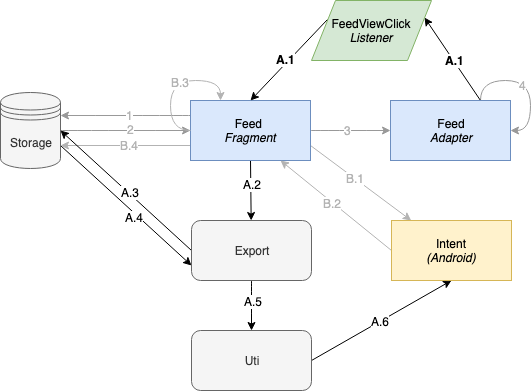
\includegraphics[scale=0.6]{images/Sharing_ImpA.png}
    \caption{Implementation of sharing functionality (A): Exporting one or all Records}
    \label{fig:impl_sharingA}
\end{figure}

\subsubsection{Action A: Exporting one or all Records}
In Figure \ref{fig:impl_sharingA}, an illustration of the steps to export one single recording is shown. However, the \verb|Feed Fragment| has an option to export all record; therefore, by disregarding the first step (A.1), the same structure applies to export all records. In essence, exporting consists of bundling the records and corresponding samples into a formated file, and prompting the user with options to select a media (e.g., mail) for transmittion. The steps can be narrowed down to: 

\begin{itemize}
    \item[A.1] Upon an event for exporting a selected record in \verb|Feed Adapter|, the record information is sent to the \verb|Feed Fragment| through the callback reference (\verb|onRecordAnalyticsClick|) between these components. The record information will be used to determine the corresponding samples for the record.
    \item[A.2] The \verb|Feed Fragment| delegates record information to the \verb|export| method inside of the \verb|Export| class. The class is responsible for enabling exportation. 
    \item[A.3] An operation to retrieve all samples related to the record with the use of the \verb|SampleViewModel| is done. 
    \item[A.4] The \verb|export| method retrieves all of the samples related to the record. Next, the record and the samples are encoded into an exportable JSON format (Ref: Data Format). To enable the sharing interface provided by Android, the content has to be stored on the device. Thus, the encoded data is written into a file on the device, with a filename of \verb|record_(current_date).json|, and the next component uses the reference to the file location. 
    \item[A.5] The encoded file is retrieved with the use of \verb|FileProvider| (facilitates secure sharing of files [ref]). The code for this step are
\begin{lstlisting}[language=json, caption={My Caption}, captionpos=b]
static void shareFileIntent(Activity a, File file) {

    Uri fileUri = FileProvider.getUriForFile(a.getApplicationContext(), a.getApplicationContext().getPackageName() + ".provider", file);

    Intent iShareFile = new Intent(Intent.ACTION_SEND);
    iShareFile.setType("text/*");
    iShareFile.putExtra(
        Intent.EXTRA_SUBJECT, "Share Records");
    iShareFile.putExtra(Intent.EXTRA_STREAM, fileUri);
    ...

    a.startActivity(
        Intent.createChooser(iShareFile, "Share Via"));
}

\end{lstlisting}

    \item[A.6] The user is displayed with a popup interface with several options to share the file over a media. An illustration of the layout can be found in Section Representation. 


\end{itemize}


\begin{figure}
    \centering
    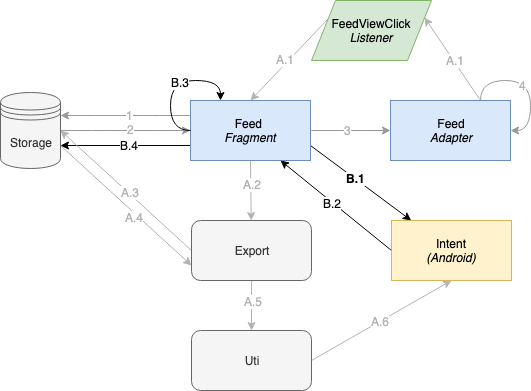
\includegraphics[scale=0.6]{images/Sharing_ImpB.png}
    \caption{Implementation of sharing functionality (B)}
    \label{fig:impl_sharingB}
\end{figure}

\subsubsection{Action B: Import a Record from the Device}
In Figure \ref{fig:impl_sharingB}, an illustration of importing a record from the device is shown. Importing conists of locating the formated file (the user has to obtain the file and store it on the device on beforehand), parsing the content in the file, and storing the data respective to the users database. The steps can be narrowed down to:

\begin{itemize}
    \item[B.1] The user requests to view the import record interface. The interface is provided by Android, and allows the user to select particular kind of data on the device (ref). The code for this action is:
\begin{lstlisting}[language=json, caption={My Caption}, captionpos=b]
private void importRecords() {
    Intent intent = new Intent(Intent.ACTION_GET_CONTENT);
    intent.setType("*/*");
    startActivityForResult(intent, 1);
}

\end{lstlisting}
    \item[B.2] Once the user has selected the desired file, the method \verb|onActivityResult| inside of \verb|Feed Fragment| is called, and location of the selected file can be located. 
    \item[B.3] The file location is an obscured path to the file on the device; thus, parsing the path with the use of \verb|Cursor| method has to be done. After the absolute path is found, the data is decoded accordingly to the data format, and the records are sent back to \verb|Feed Fragment|.
    \item[B.4] The necessary record information and the samples are extracted from the decoded data, and are inserted into the users database. 
\end{itemize}

\subsection{Modules}
Modules are standalone application, that provides data enrichment and extended functionality to the application. The modules leverages the records and samples to analyze, evalutate or detect sleeping disorders. In order to add and launch a module in Nidra, we need the modules package name. The package name and the name of the module-application can be obtained in Android. Thus, the actions to enable modules in the application are: (A) add a module; and (B) launch a module. 

Before a user can take these actions, the records from the database have to be presented. The \verb|Feed Fragment| contains a \verb|RecyclerView| which populates the records into inside the \verb|Feed Adapter| (steps: 1-4). The adapter contains all the interactions and the event handling (i.e., button event listener for exporting) for a single record. 

In this Subsection, we will take a look into the steps that are taken to enable the actions.

\subsubsection{Action A: Add a Module}
In order to add a new module, the user has to install the module-application on the device on beforehand. By listing through the installed application on the device, the user can select the desired module to be added in Nidra. In Figure \ref{fig:impl_modulesA}, an illustration of adding a module is shown, and the steps can be narrowed down to:

\begin{figure}
    \centering
    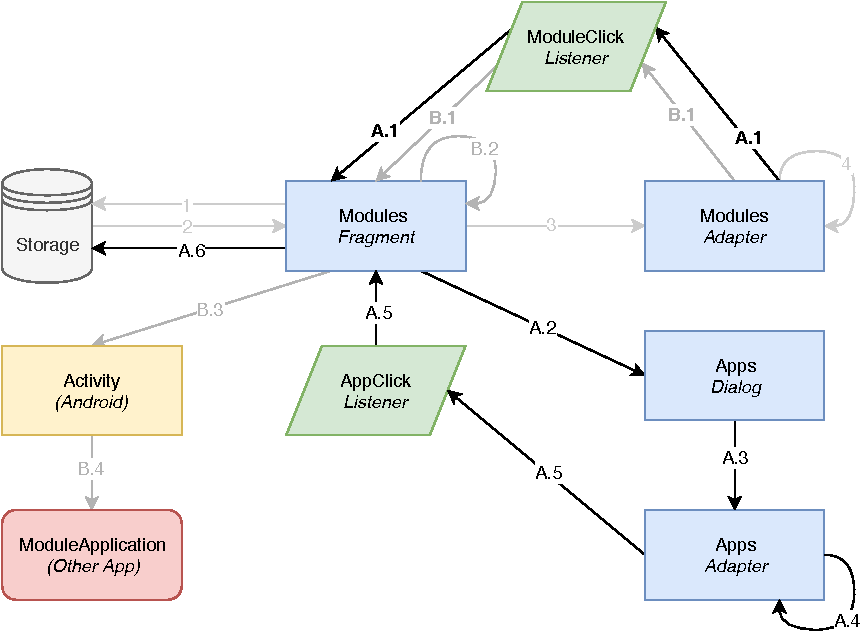
\includegraphics[scale=0.7]{images/Module_ImpA.pdf}
    \caption{Implementation of module functionality(A): Add a Module}
    \label{fig:impl_modulesA}
\end{figure}

\begin{itemize}
    \item[A.1] Upon an event for adding a new module in \verb|Modules Adapter|, the \verb|Feed Fragment| is notified through the callback reference (\verb|onNewModuleClick|) between these components.
    \item[A.2] The \verb|Modules Fragment| lauches a custome Android dialog, which will list all of the installed application on the device. 
    \item[A.3] The \verb|Apps Adapter| will fetch all of the application that is not a system package, already installed module, or the current application (Nidra). Next, the the adapter for the dialog will be populated with the eligible applications. 
    \item[A.4] Once the user has selected the desired module-application, an event to the \verb|Modules Fragment| through the callback reference \verb|onAppItemClick| between these components are made. The callback contains an object with the \verb|PackageInfo| for the selected module-application.
    \item[A.5] The dialog is dismissed, and the application name and packagename are extracted from the \verb|PackageInfo| for the selected module-application. 
    \item[A.6] Furthermore, the acquired information is stored in our database for modules through the DAO interface. 
\end{itemize}

\subsubsection{Action B: Launch a Module}
A module is launched in a seperate process, due to Android prohibits launching for other applications inside of an application. All added modules are listed and presented to the user in a separate screen, and on launch of a module, all of the data that Nidra obtains from recordings, are encoded into a JSON format and bundled with the launch of the module. In Figure \ref{fig:impl_modulesB}, an illustration of launching a module, and the steps can be narrowed down to:

\begin{figure}
    \centering
    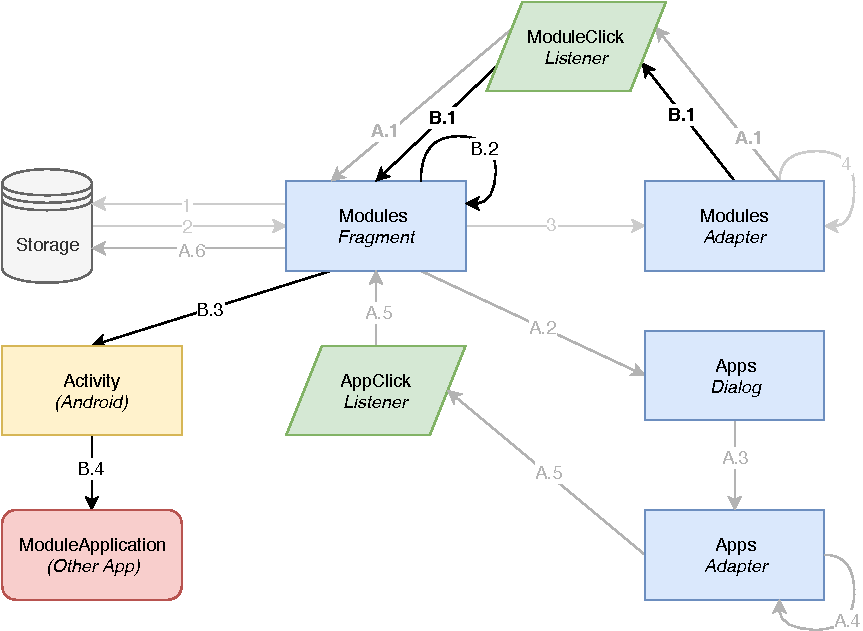
\includegraphics[scale=0.7]{images/Module_ImpB.pdf}
    \caption{Implementation of module functionality(B): Launch a Module}
    \label{fig:impl_modulesB}
\end{figure}

\begin{itemize}
    \item[B.1] Upon an event for launching a module in \verb|Module Adapter|, the packagename of the module is sent to the \verb|Modules Fragment| through the callback reference (\verb|onLaunchModuleClick|) between these components. The packagename  will be used to launch the module-application.
    \item[B.2] All of the records and samples on the device for the user, is bundled and formated into a JSON, and launched:
\begin{lstlisting}[language=json, caption={My Caption}, captionpos=b]
public void onLaunchModuleClick(String packageName) {
    Intent moduleApplication = context.getPackageManager().getLaunchIntentForPackage(packageName);

    if (moduleApplication == null) return;

    String data = formatAllRecordsToJSON();

    Bundle bundle = new Bundle();
    bundle.putString("data", data);

    moduleApplication.putExtras(bundle);

    startActivity(moduleApplication);
}
\end{lstlisting}

    \item[B.3] The activity uses the data provided in the \verb|Intent| that includes the packagename (the name of the module-application to determine the correct application).
    \item[B.4] The selected module is then launched, and presented to the user. The user can at anytime press the back button, to return to Nidra.  
\end{itemize}

%\begin{figure}
%    \centering
%    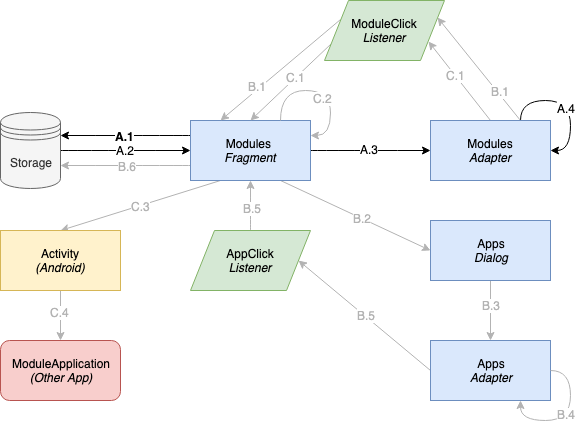
\includegraphics[scale=0.6]{images/Module_ImpA.png}
%    \caption{Implementation of module functionality(A)}
%    \label{fig:impl_modulesA}
%\end{figure}



%\subsubsection{Data Exchange Implementation}


\begin{figure}
    \centering
    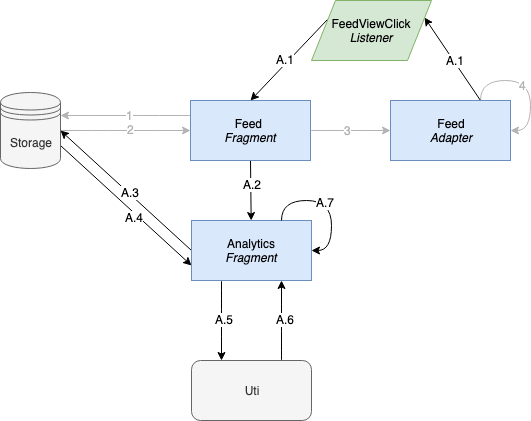
\includegraphics[scale=0.6]{images/Anal_Imp.png}
    \caption{Implementation of analytics functionality (A): Display a Graph for a Single Record}
    \label{fig:impl_analytics}
\end{figure}

\subsection{Analytics}
Analytics is the part of illustrating and analyzing the records. In Nidra, the analytics part of the implementation is limited to a time-series graph for a single record. However, there are possibilities of extending the \verb|Analytics Fragment| with other graphs based on the current structure. The current action for analytics is A) display a graph for a single record to the user. 

Similar to sharing, the records from the database have to be presented. The \verb|Feed Fragment| contains a \verb|RecyclerView| which populates the records into inside the \verb|Feed Adapter| (steps: 1-4). The adapter contains all the interactions and the event handling (i.e., button event listener for analytics) for a single record. 

In this Subsection, we will take a look into the steps that are taken to enable the action.

\subsubsection{Action A: Display a Graph for a Single Record}
Nidra provides a simple time-series graph of respiration data obtained during the recording. The graph data is plotted into a Library, which enables interactions (e.g., zoom and scrolling) on the data. The X-axis is the respiration value based on the Y-axis time of sampling. In Figure \ref{fig:impl_analytics}, an illustration of displaying a graph shown. The steps can be narrowed down to:

\begin{itemize}
    \item[A.1] Upon an event for analytics on a selected record in \verb|Feed Adapter|, the record information is sent to the \verb|Feed Fragment| through the callback reference (\verb|onRecordAnalyticsClick|) between these components. The record information will be used to determine the corresponding samples for the record.
    \item[A.2] A new instance of the \verb|Analytics Fragment| is created, and an transition from the \verb|Feed Fragment| to the \verb|Analytics Fragment| is made. Alongside, the record information is transmitted.
    \item[A.3] An operation to retrieve all samples related to the record with the use of the \verb|SampleViewModel| is done. 
    \item[A.4] The \verb|Analytics Fragment| retrieves all of the samples related to the record. The samples has to be structured according to the graph library to display an interactive time-series graph. (GraphView (ref)).
    \item[A.5] Each sample has to be extracted from the sample-data, acccordingly to the sensor data structure.
    \item[A.6] The sample value is returned, and inserted into an array over datapoints used in the graph. 
    \item[A.7] The use is presented with a graph, which is interactable. The Y-axis has the sample value on given time (in HH:MM:SS) on the X-axis. The graph library enables interactions (e.g., zooming and scrolling) the user can do, to gain a better understanding of the recording. 
\end{itemize}



\subsection{Storage}
\begin{figure}
    \centering
    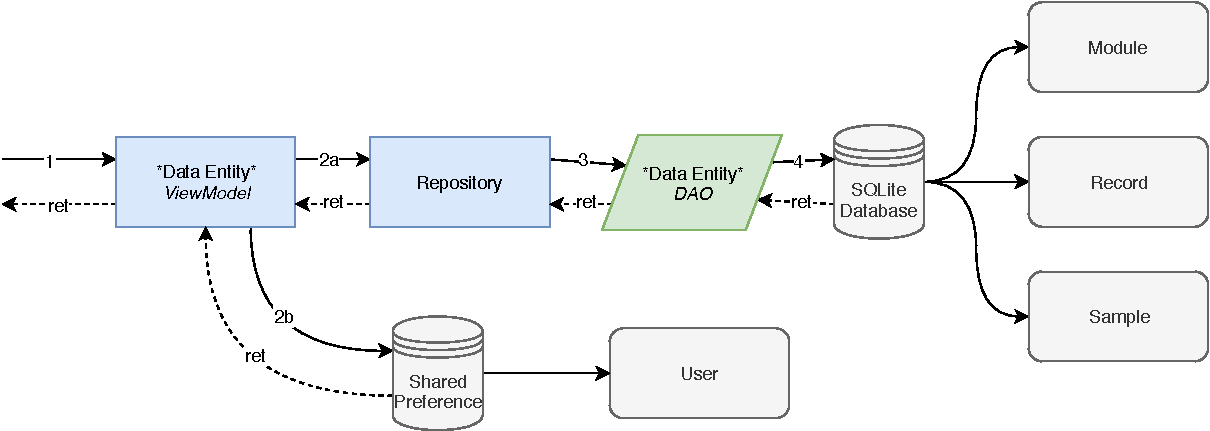
\includegraphics[scale=0.60]{images/Storage_Imp.pdf}
    \caption{Entity Relationship Diagram}
    \label{fig:impl_storage}
\end{figure}


Storage facilities persistent data which remain available after application termination. In Nidra, there are four individual data entities (i.e., record, sample, module, and user). In the Subsection about Data Entities, we discussed the design choices of the individual data entity. The standard CRUD operations on each data entities are: insert, update, and delete. Also, the user has an operation to retrieve the biometrical data, module and record have an operation to retrieve all of the entries in the database, and samples have an operation to retrieve all of the entries corresponding to a record. 

Android Room provides an abstract layer over SQLite to enable easy database access [Cite]. In Figure \ref{fig:impl_storage}, the flow for accessing and retrieving the data from the database based on the Android Room architecture is shown and can be described as:

\begin{itemize}
	\item[1] Each data entity has a \verb|ViewModel| where all of the CRUD operation (e.g., insert, update, delete, or retrieve) goes through.  A view model is designed to store and manage UI-related data in a conscious way, that allows data to be persistent through configuration changes (e.g., screen rotations) [CITE]. 
 	\item[2a] The predefined operations point to the repository. Repository modules handle data operations and provide an API  which makes data access easy. A repository is a mediator between different data sources (e.g., database, web services, and cache) [CITE]. In Nidra, the only data source is the database, but repository facilities future data sources. 
	\item[2b] The storage of the user is not in the database; however, in a \verb|SharedPreference| on the device. Shared preference points to a file containing key-value pairs and provides methods to read and write. The location of the user's shared preference is \verb|no.uio.cesar.user_storage|. 
	\item[3] Each data entity (disregarding user) has a data access object (DAO), where the SQL operations to the database are defined. 
	\item[4] Based on the operation, the data is accessed and retrieved from the SQLite database.
\end{itemize}


\subsection{Presentation}
In this Subsection we will present the user-interface (UI) based on the functionality of recording, sharing, module and analytics. The interface is developed based on the design descisions of the application, as well as creating a user-interface that is simple and efficent for a user to interact with. We try to limit the actions the user can take on a screen, to make the application simpler to understand and comprehend. 

\subsubsection{UI: Recording}
\begin{figure}
    \centering
    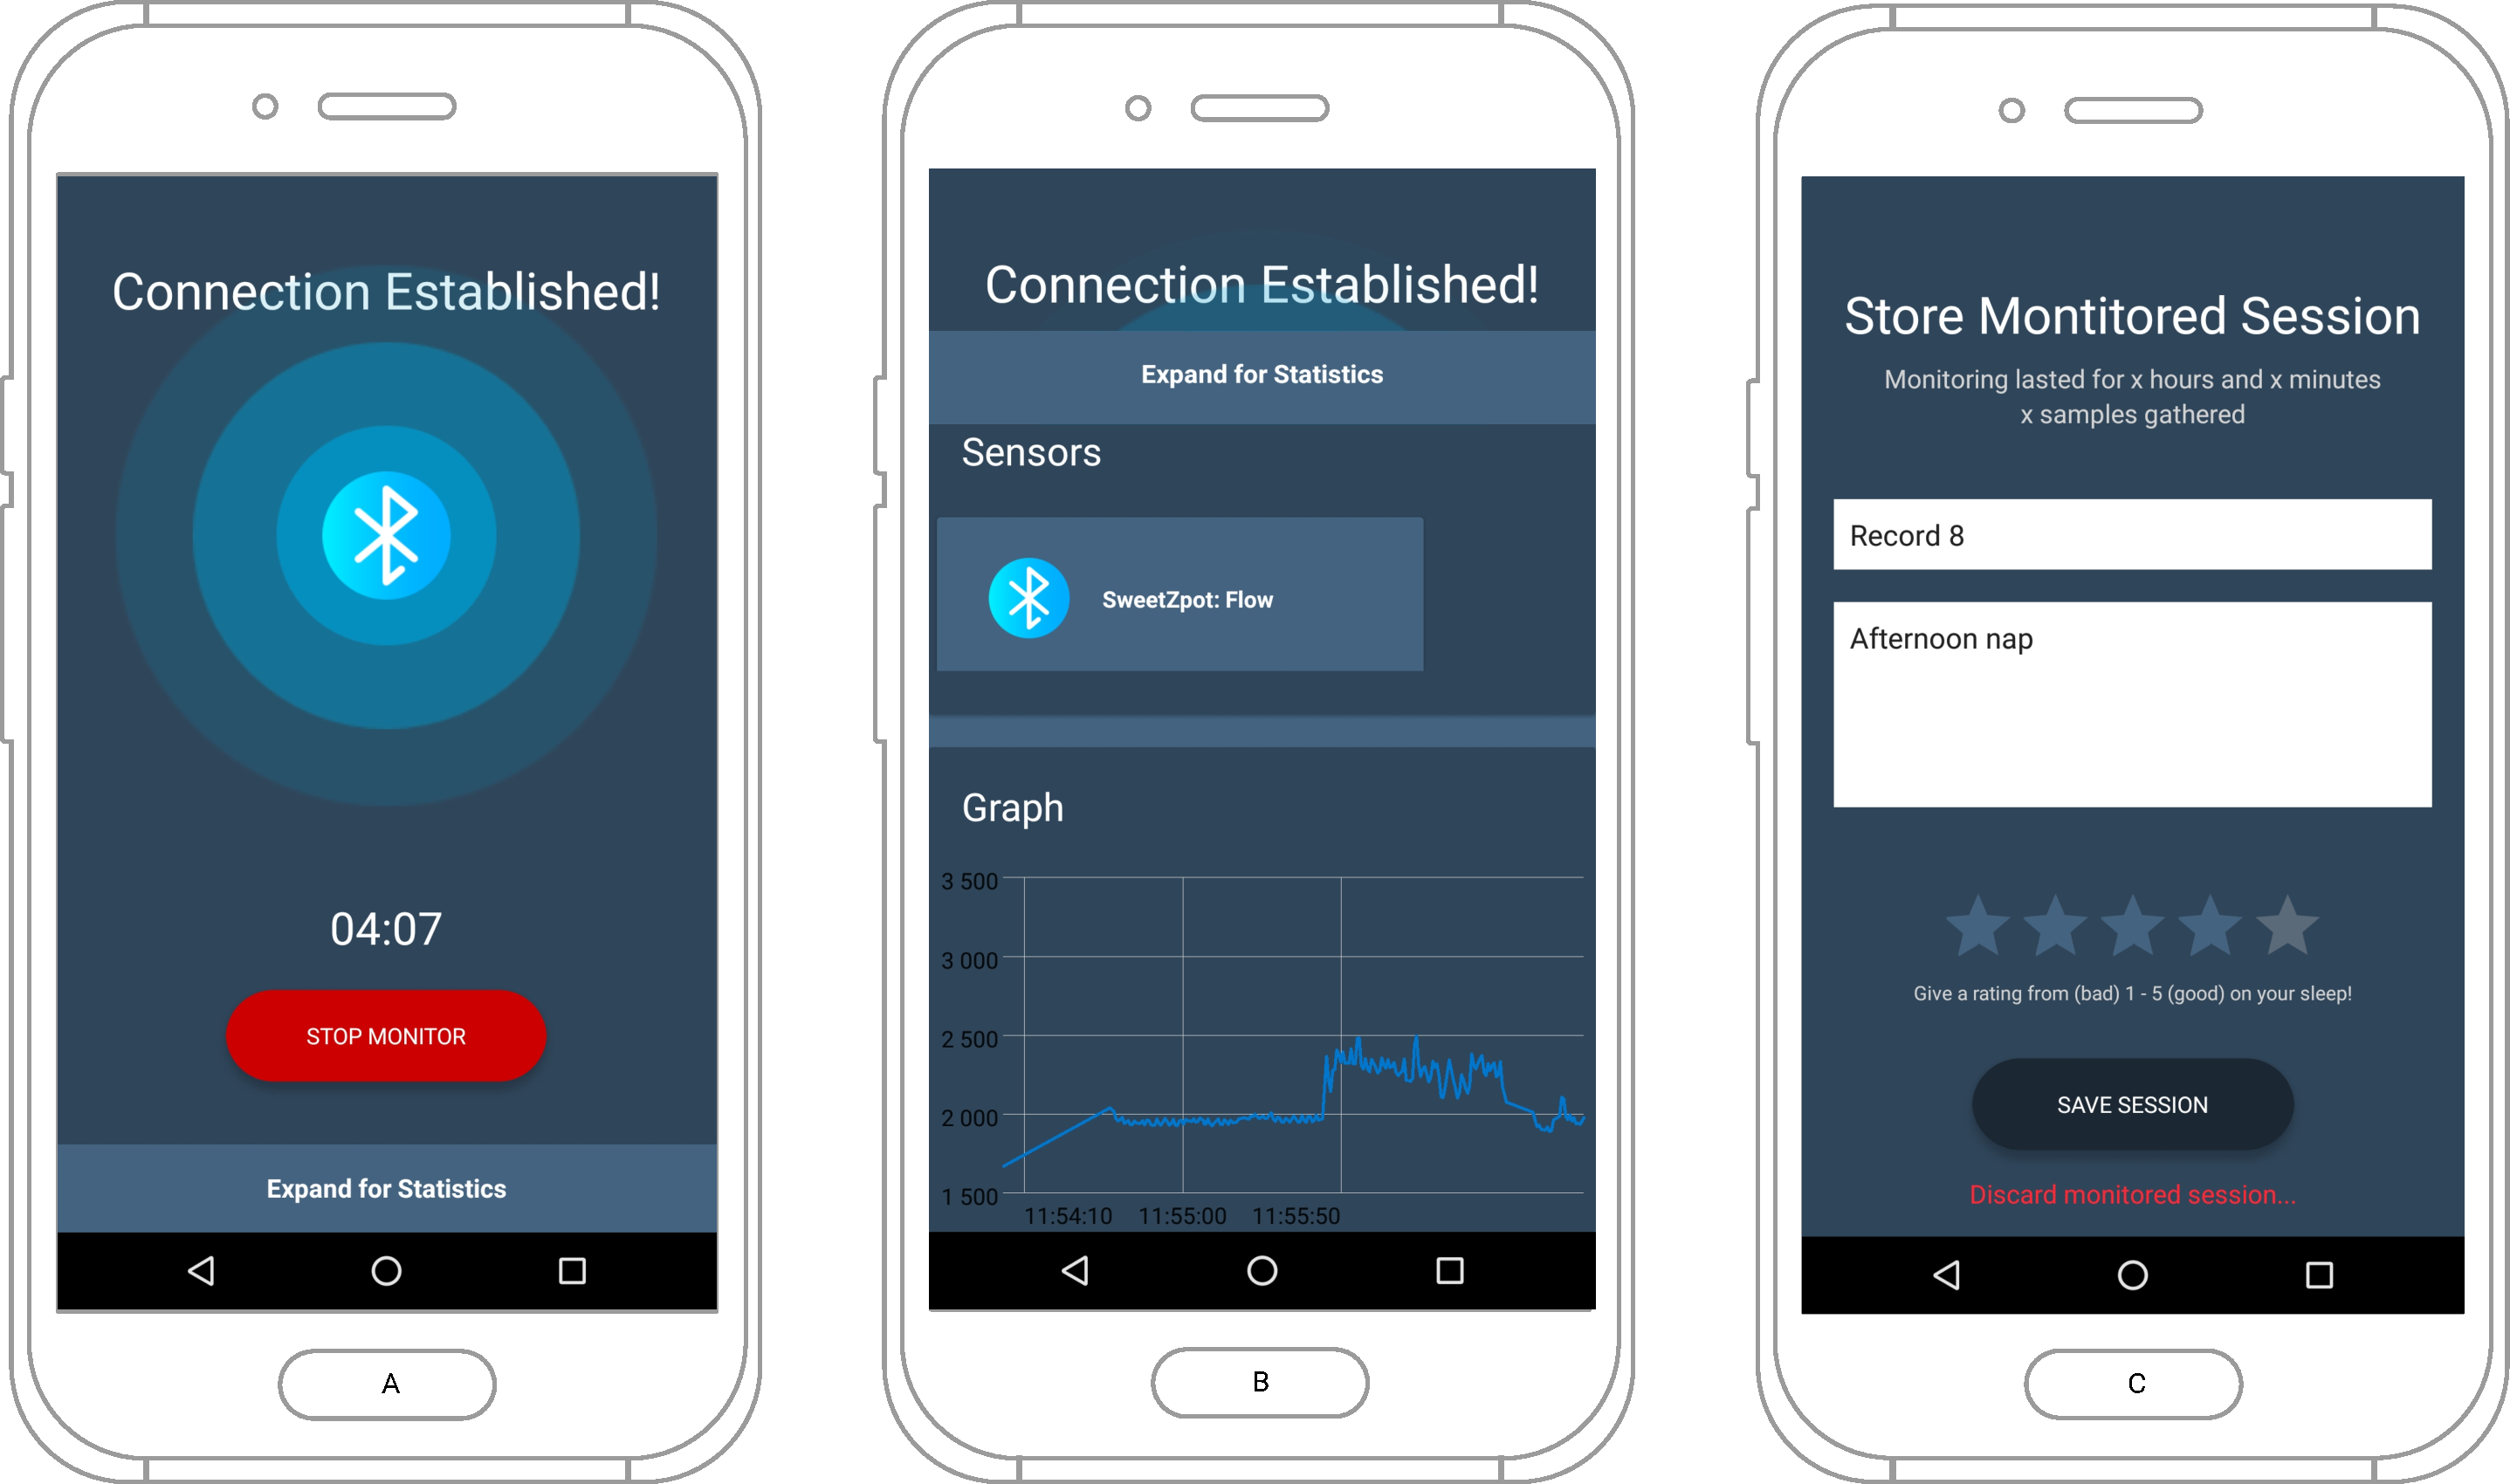
\includegraphics[scale=0.26]{images/Recording_img.pdf}
    \caption{The recording screen displayed to the user; with the screen: (A) during a recording, (B) real-time analytics, and (C) finalizing the recording}
    \label{fig:screen_recording}
\end{figure}

Figure \ref{fig:screen_recording} shows the screen for: (A) during a recording, (B) the real-time analytics, and (C) finalizing the recording. 

\begin{itemize}
    \item[A] The screen has a ripple effect to indicate the state of the recording to the user. There are two types of ripple colours; a blue ripple effect for samples acquistion, and a grey ripple effect if the sensor has disconnected. The ripple effect is only active if the screen is turned on, in order to perserve battery life. During disconnects between the sensor and the device, the user provide no extra input to resolve the issue. However, if the numbers of attempts is reached, the user is presented with the finalizing screen (C). Also, this screen display the elapsed recording time, and has a visible button to stop the recording. 
    \item[B] The user can extend the interface for viewing statistics regarding the recording session. Currently, the interface lists all of the available sensor sources, also a real-time interactable graph of respiration.
    \item[C] The finalzing screen allows users to specify the title and description of recording, to make it distingushable, in addition to giving a feedback on recording so the doctors/researchers can review it. Also, the user can give a rating between 1--5 (where 1 is bad, and 5 is good) to rate the sleeping.

\end{itemize}

\subsubsection{UI: Sharing}
\begin{figure}
    \centering
    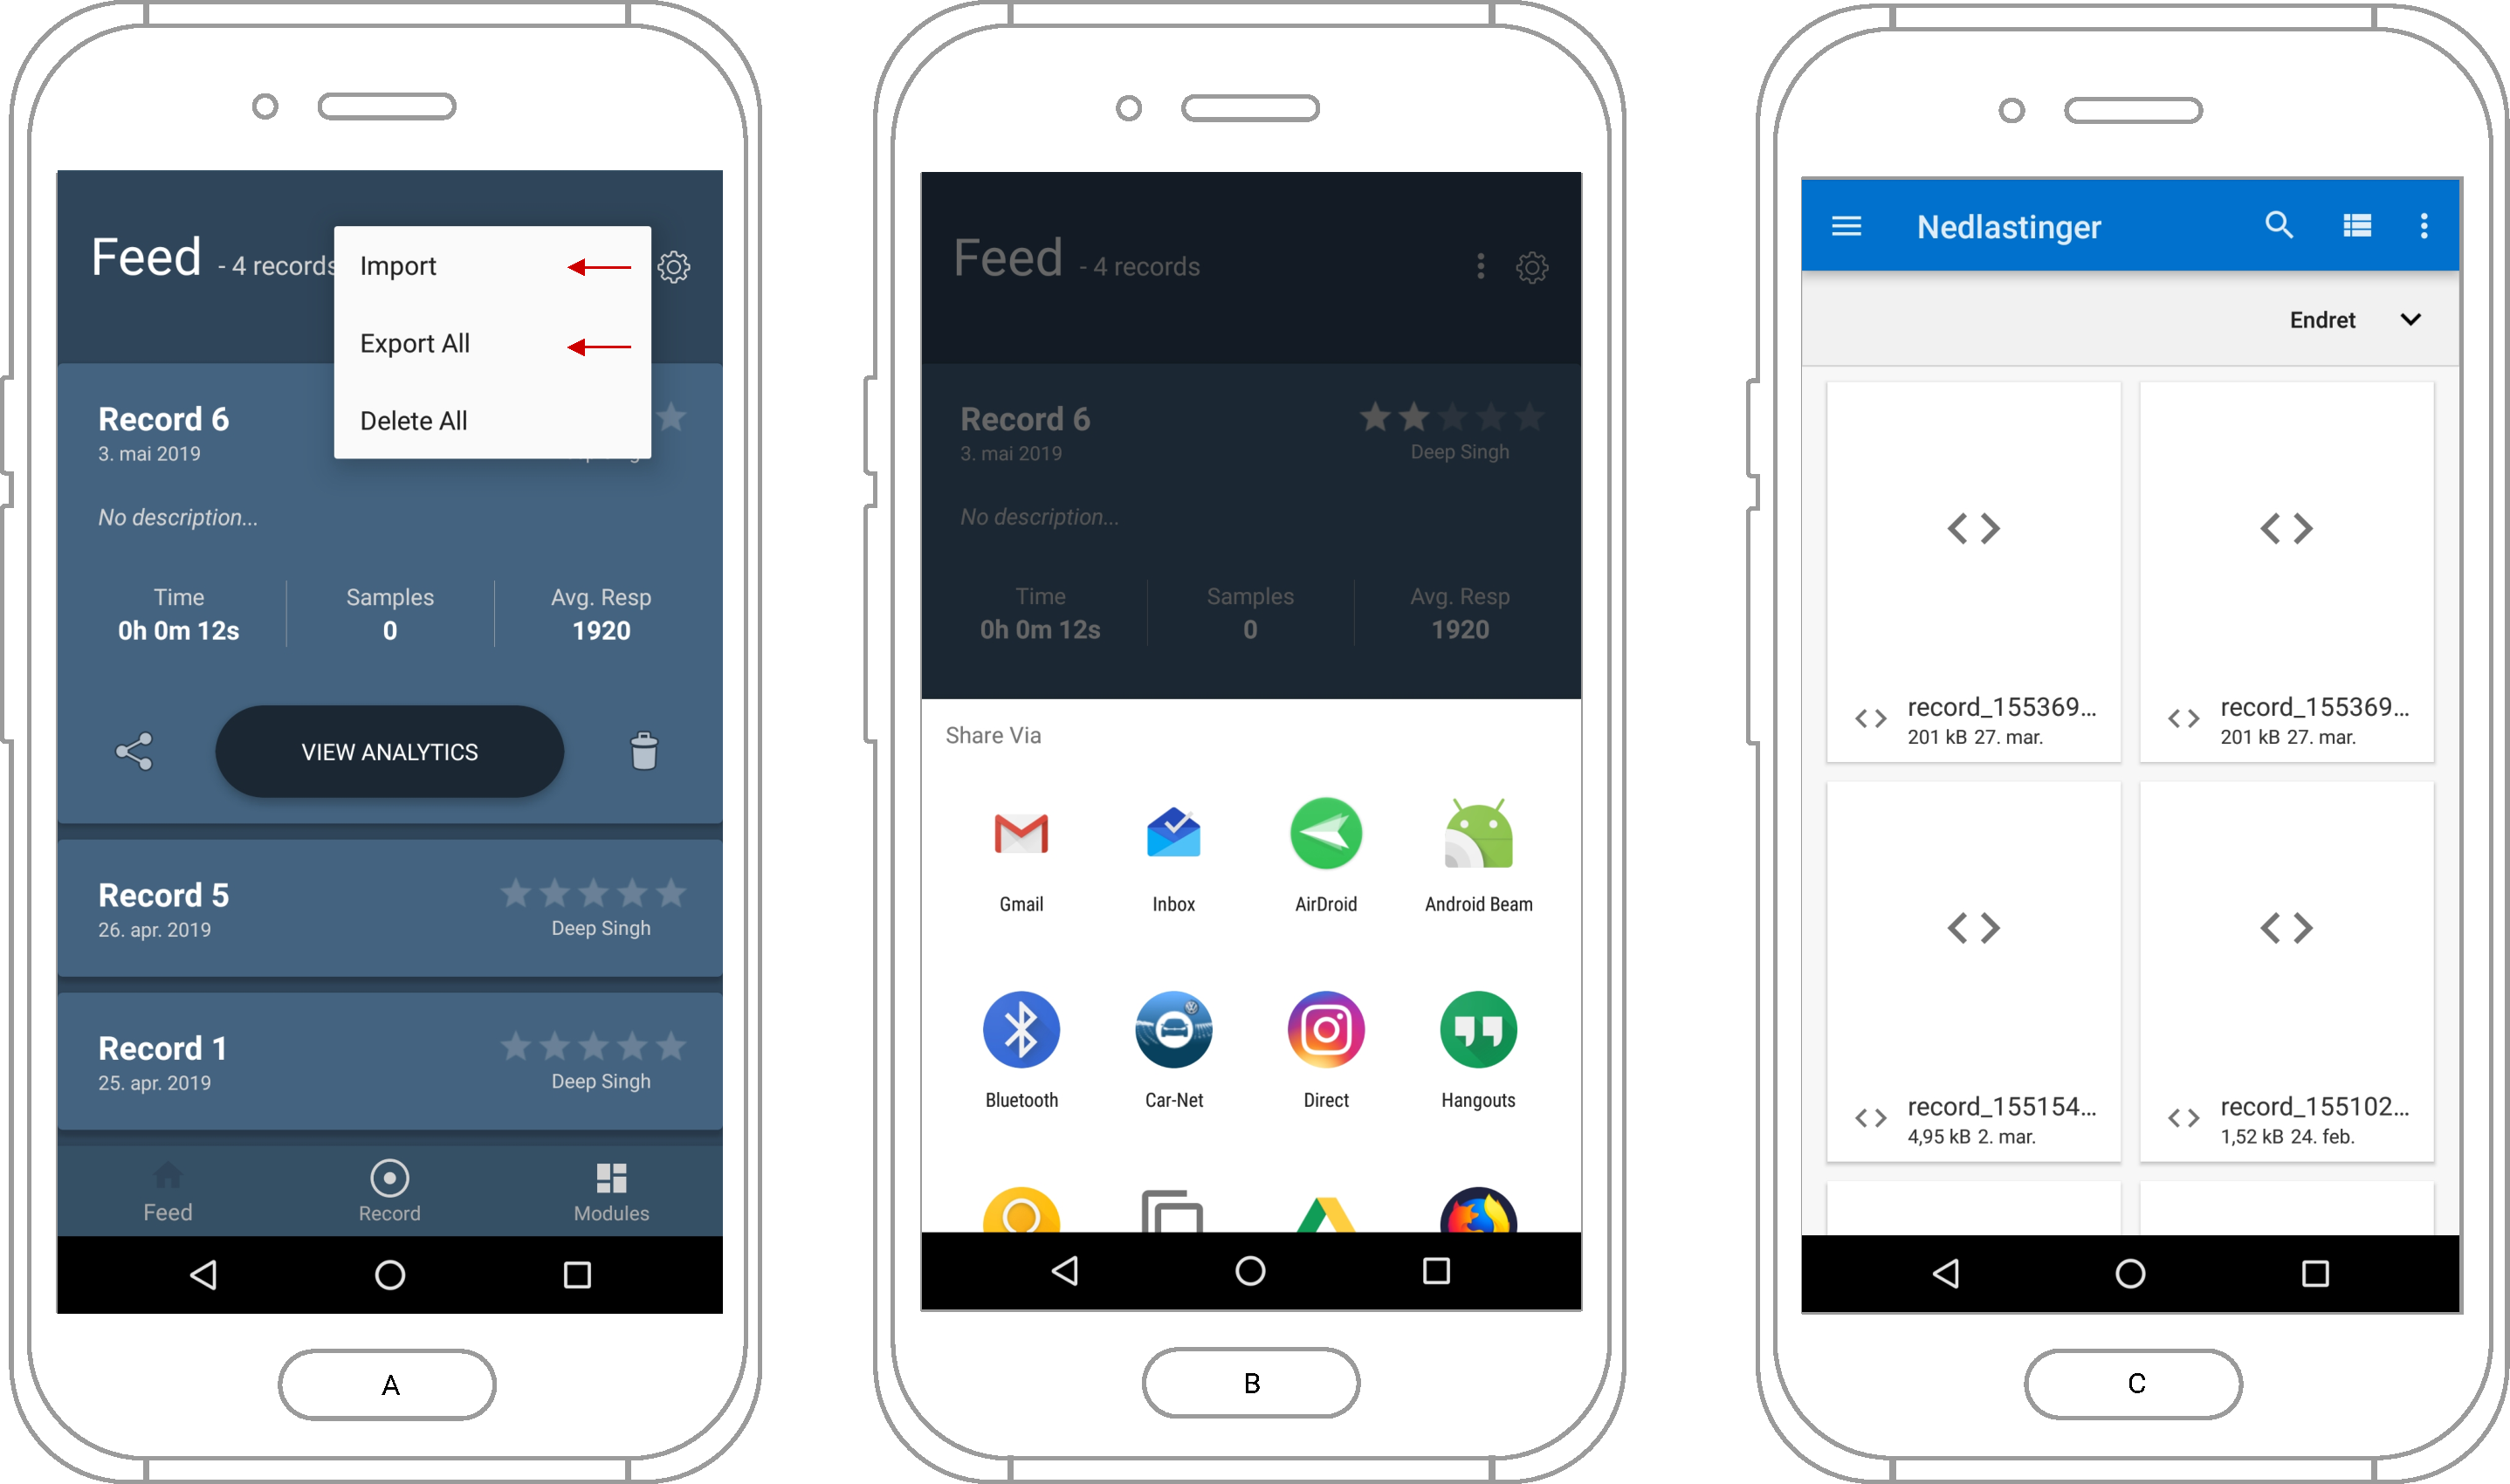
\includegraphics[scale=0.26]{images/Sharing_img.pdf}
    \caption{The sharing screen displayed to the user}
    \label{fig:screen_sharing}
\end{figure}

Figure \ref{fig:screen_sharing} shows the screen for: (A) option to import or export, (B) the media selection for exporting, and (C) the file selection for importing.

\begin{itemize}
    \item[A] The feed screen is where all of the records are presented to the user. The user can choose to export one single record, or export all. 
    \item[B] By pressing export all, an overlay with a Android provided sharing screen is presented, where the user can choose a media to export the file on. 
    \item[C] By pressing import, an overlay with downloaded files on the users device is presented. The user can press on the desired file, and the file will be parsed and added to the users collection of records.  
\end{itemize}

\subsubsection{UI: Modules}
\begin{figure}
    \centering
    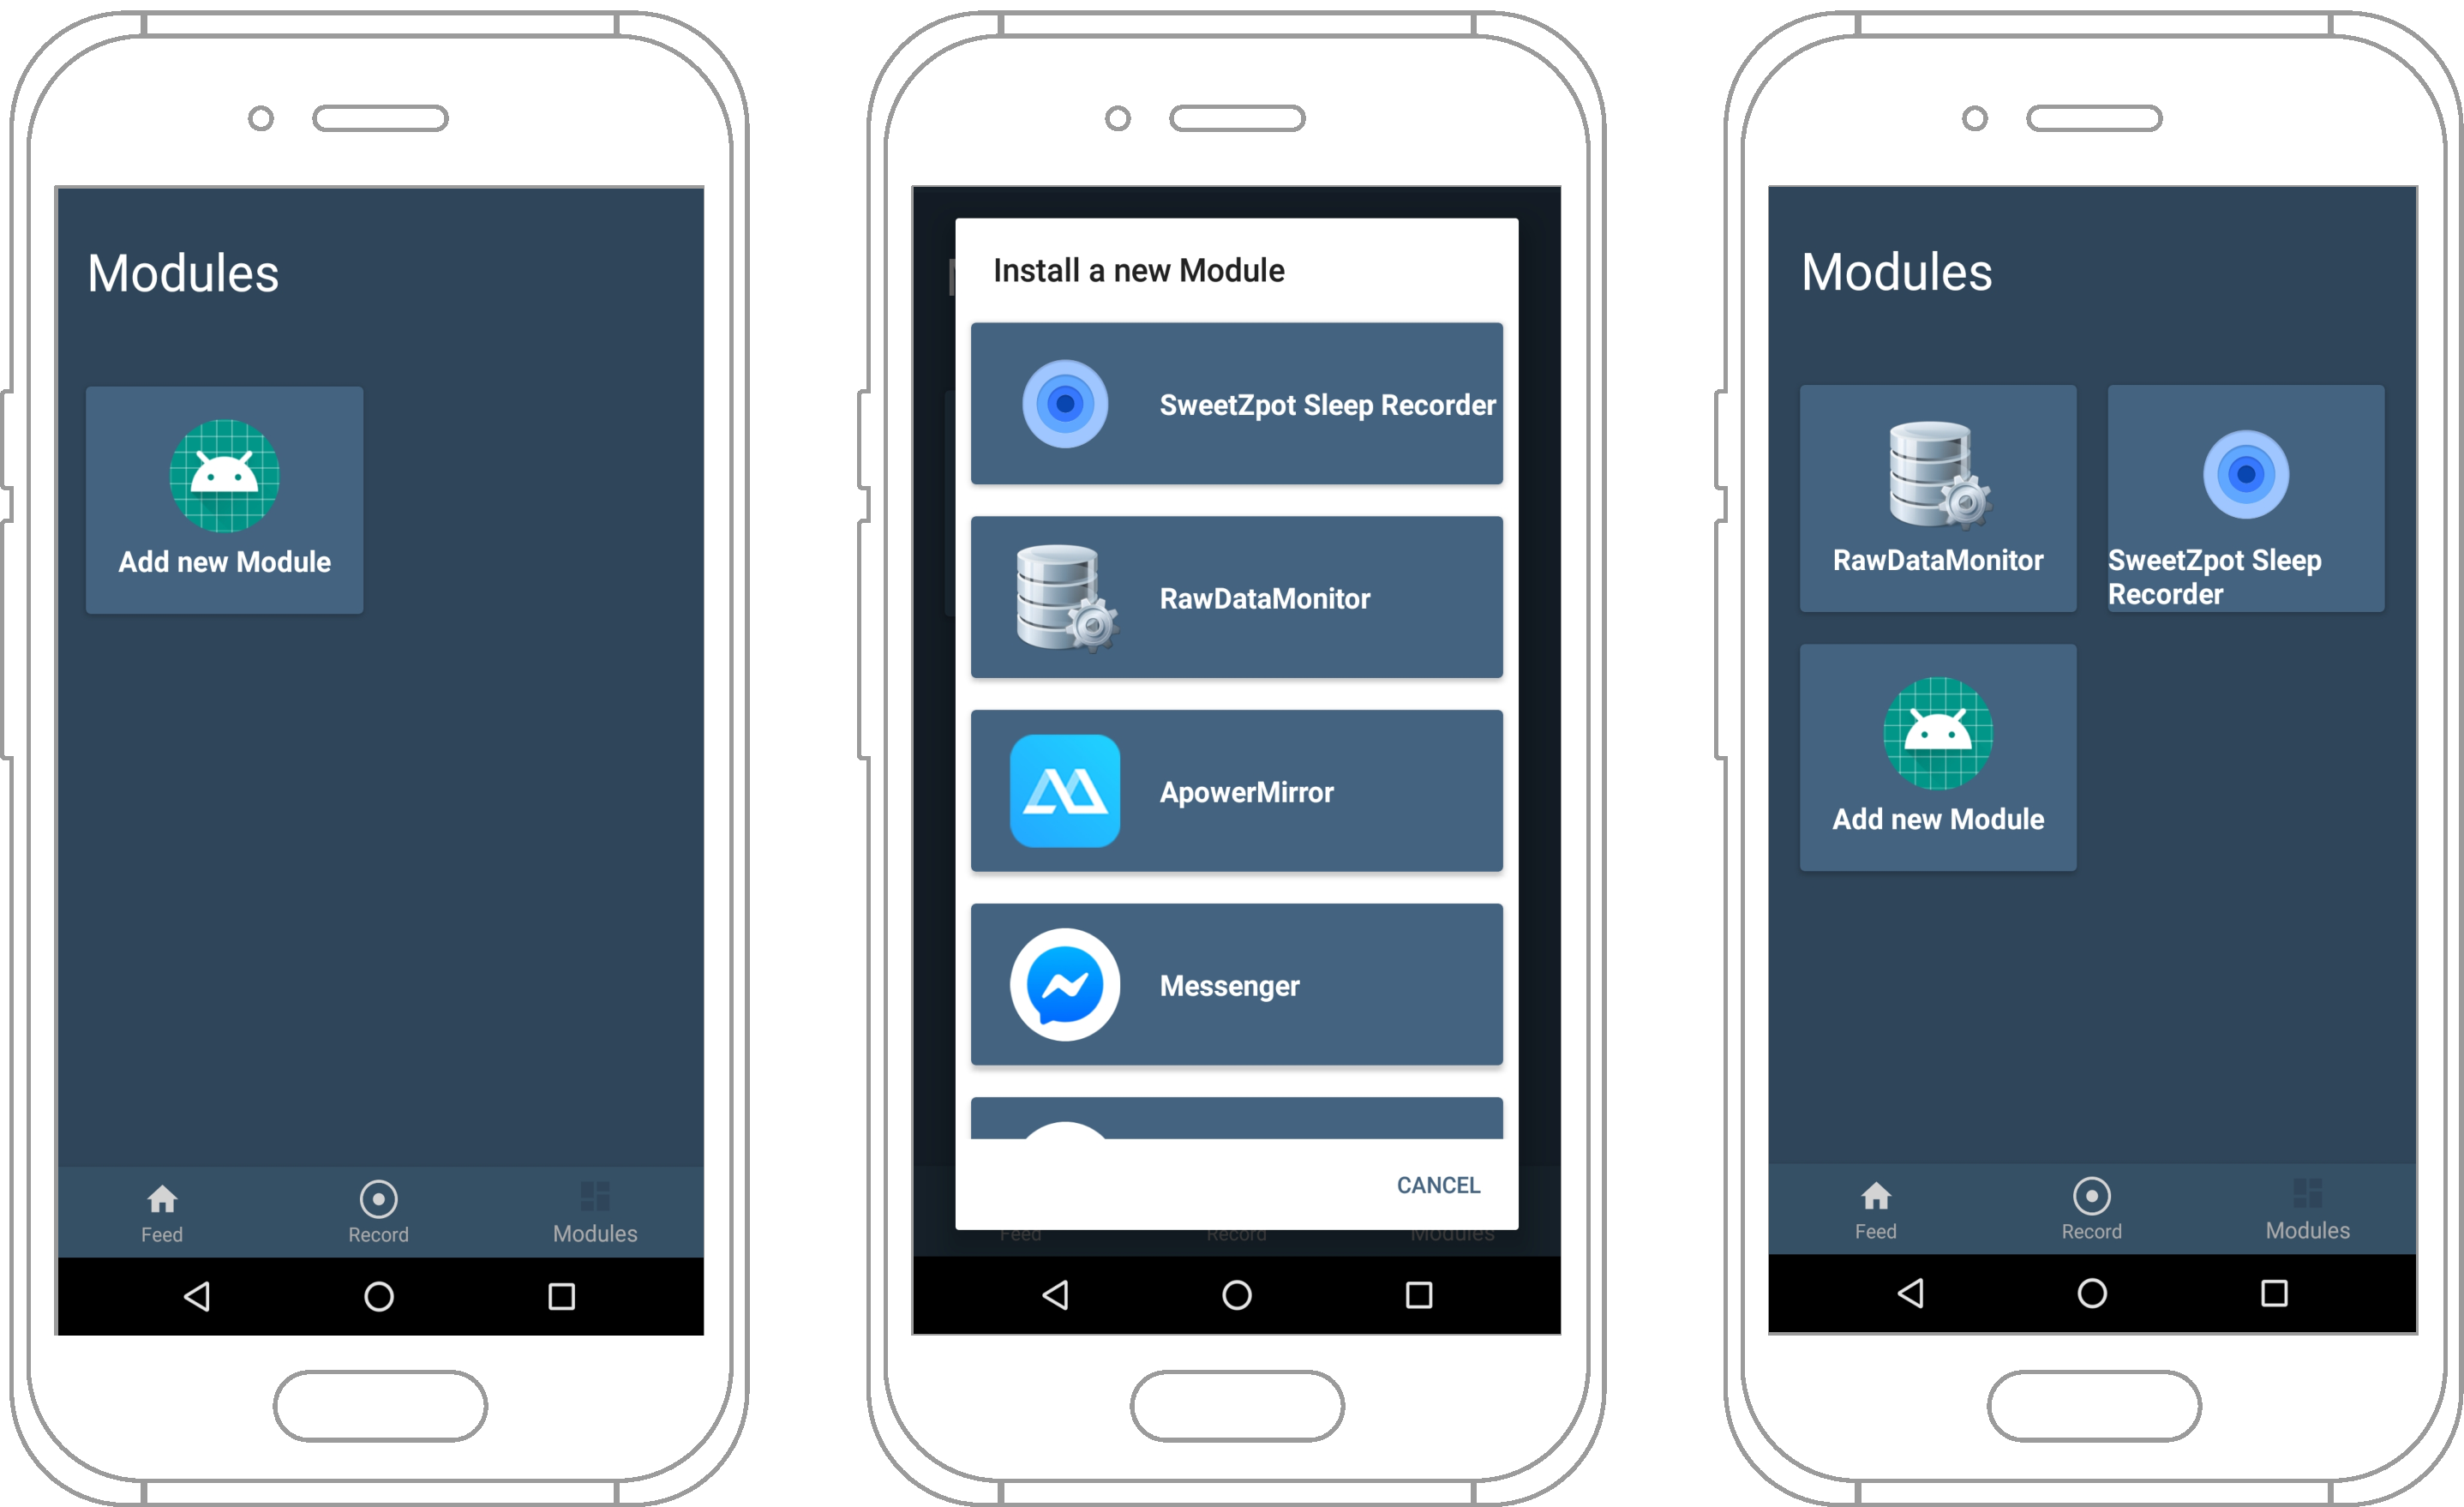
\includegraphics[scale=0.26]{images/Modules_img.pdf}
    \caption{The module screen displayed to the user}
    \label{fig:screen_modules}
\end{figure}

Figure \ref{fig:screen_modules} shows the screen for: (A) list without any modules, (B) list of installed application, and (C) list with modules. 

\begin{itemize}
    \item[A] The modules screen is shows all of the added modules to the users.
    \item[B] The user can press the \textit{add new module} button, in order to be presented with a list of all installed applications. 
    \item[C] Once the user has selected a module-application to be added in Nidra, the list of modules are updated and presented to the user.
\end{itemize}

\subsubsection{UI: Analytics}
Figure \ref{fig:screen_analytics} shows the screen for: (A) single record in the list, and (B) the analytics for the record

\begin{itemize}
    \item[A] The user can expend records in order to view more functionality and statistics of the record. One of the functionalities are to view the analytics of the record.
    \item[B] An interactable graph is presented to the users, and the graph is populated with the samples obtained from the recording for selected records. The graph shows the respiration value (Y-axis) on given time (X-axis) of sampling. 
\end{itemize}

\begin{figure}
    \centering
    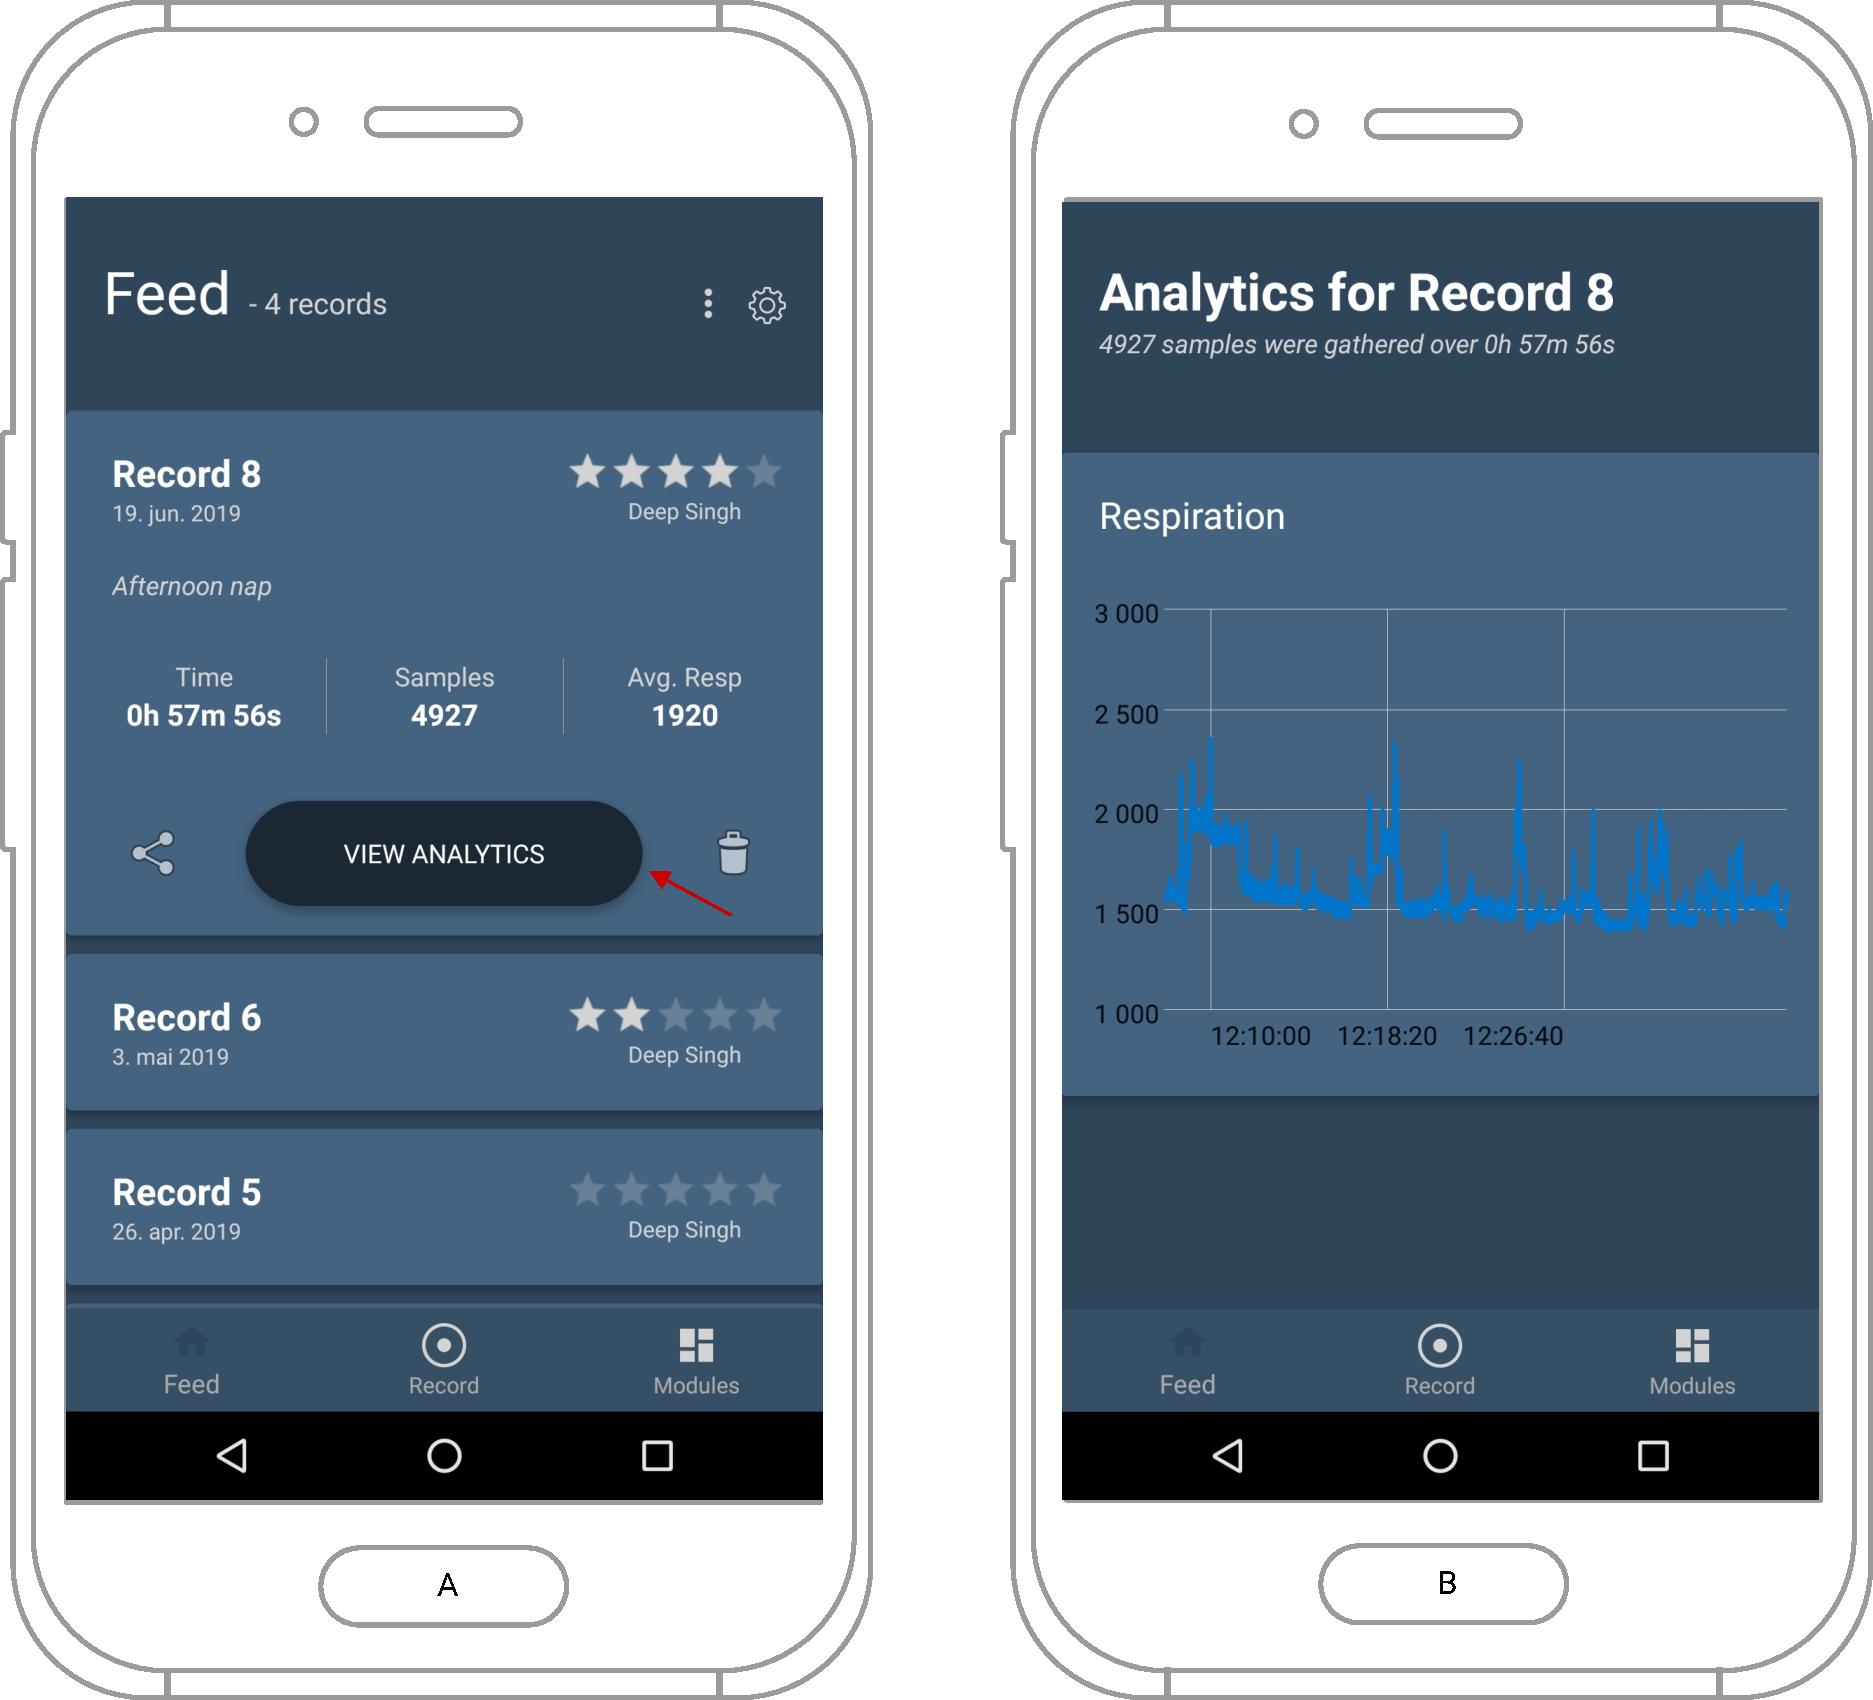
\includegraphics[scale=0.26]{images/Analytics_img.pdf}
    \caption{The analytics screen displayed to the user}
    \label{fig:screen_analytics}
\end{figure}
